% contribution.tex -- solution-overview figure.
\documentclass[tikz,border=3pt]{standalone}
\usepackage[dvipsnames]{xcolor}
\usetikzlibrary{arrows.meta,positioning,fit,calc}
\newcommand{\PredWR}{\mathsf{PredWR}}
\newcommand{\PredRW}{\mathsf{PredRW}}
\newcommand{\match}{\Delta}
\begin{document}
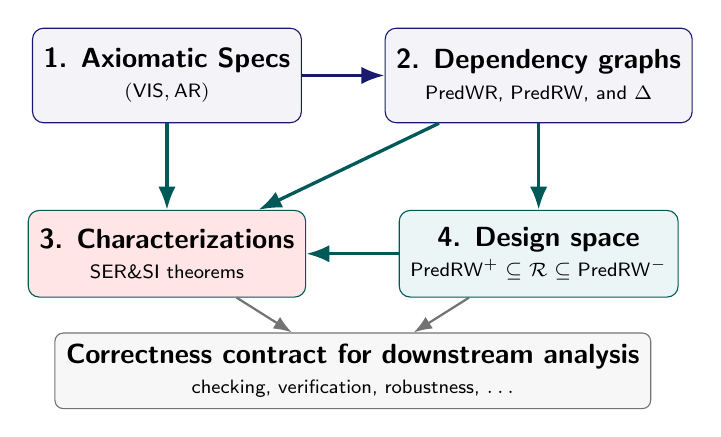
\begin{tikzpicture}[
  >=Latex,font=\sffamily,
  box/.style={draw=MidnightBlue,rounded corners=4pt,fill=MidnightBlue!5,
    align=center,minimum width=3.35cm,minimum height=1.2cm,inner sep=4pt},
  result/.style={draw=teal!70!black,rounded corners=4pt,fill=teal!8,
    align=center,minimum width=3.25cm,minimum height=1.1cm,inner sep=4pt}]
  \node[box] (spec) {\textbf{1. Axiomatic Specs}\\[-1pt]\scriptsize $(\mathsf{VIS}, \mathsf{AR})$};
  \node[box,right=1.05cm of spec] (dep) {\textbf{2. Dependency graphs}\\[-1pt]\scriptsize $\PredWR$, $\PredRW$, and $\match$};
  \draw[-Latex,very thick,MidnightBlue] (spec) -- (dep);
  \node[result,fill=red!10,below=1.10cm of spec] (theorem) {\textbf{3. Characterizations}\\[-1pt]\scriptsize SER\&SI theorems};
  \node[result,below=1.10cm of dep] (space) {\textbf{4. Design space}\\[-1pt]\scriptsize $\PredRW^+\subseteq\mathcal R\subseteq\PredRW^-$};
  \draw[-Latex,very thick,teal!70!black] (spec) -- (theorem);
  \draw[-Latex,very thick,teal!70!black] (space) -- (theorem);
  \draw[-Latex,very thick,teal!70!black] (dep) -- (theorem);
  \draw[-Latex,very thick,teal!70!black] (dep) -- (space);
  \node[draw=black!55,rounded corners=3pt,fill=black!3,align=center,
    below=1.00cm of $(theorem)!0.5!(space)$,minimum width=6.7cm,inner sep=4pt] (use) {\textbf{Correctness contract for downstream analysis}\\[-1pt]\scriptsize checking, verification, robustness, $\ldots$};
  \draw[-Latex,thick,black!55] (theorem) -- (use);
  \draw[-Latex,thick,black!55] (space) -- (use);
\end{tikzpicture}
\end{document}
